% Auto-generated by scripts/build_ch5_evidence_tables.py from outputs/analysis/chm_judged.json (2026-10-19).
\begin{figure}[!htbp]
\centering
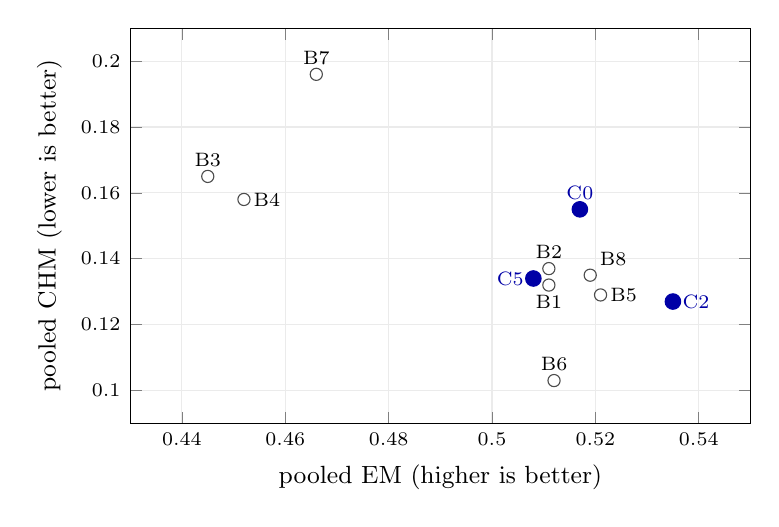
\begin{tikzpicture}
\begin{axis}[width=0.78\textwidth, height=6.6cm, xlabel={pooled EM (higher is better)}, ylabel={pooled CHM (lower is better)},
  xmin=0.43, xmax=0.55, ymin=0.09, ymax=0.21, font=\small, tick label style={font=\scriptsize}, grid=major, grid style={black!8}]
  \addplot[black!70, only marks, mark=o, mark size=2.2pt] coordinates {(0.511,0.132)};
  \node[font=\scriptsize, anchor=north] at (axis cs:0.511,0.132) {B1};
  \addplot[black!70, only marks, mark=o, mark size=2.2pt] coordinates {(0.511,0.137)};
  \node[font=\scriptsize, anchor=south] at (axis cs:0.511,0.137) {B2};
  \addplot[black!70, only marks, mark=o, mark size=2.2pt] coordinates {(0.445,0.165)};
  \node[font=\scriptsize, anchor=south] at (axis cs:0.445,0.165) {B3};
  \addplot[black!70, only marks, mark=o, mark size=2.2pt] coordinates {(0.452,0.158)};
  \node[font=\scriptsize, anchor=west] at (axis cs:0.452,0.158) {B4};
  \addplot[black!70, only marks, mark=o, mark size=2.2pt] coordinates {(0.521,0.129)};
  \node[font=\scriptsize, anchor=west] at (axis cs:0.521,0.129) {B5};
  \addplot[black!70, only marks, mark=o, mark size=2.2pt] coordinates {(0.512,0.103)};
  \node[font=\scriptsize, anchor=south] at (axis cs:0.512,0.103) {B6};
  \addplot[black!70, only marks, mark=o, mark size=2.2pt] coordinates {(0.466,0.196)};
  \node[font=\scriptsize, anchor=south] at (axis cs:0.466,0.196) {B7};
  \addplot[black!70, only marks, mark=o, mark size=2.2pt] coordinates {(0.519,0.135)};
  \node[font=\scriptsize, anchor=south west] at (axis cs:0.519,0.135) {B8};
  \addplot[blue!65!black, only marks, mark=*, mark size=2.8pt] coordinates {(0.517,0.155) (0.535,0.127) (0.508,0.134)};
  \node[font=\scriptsize, anchor=south, text=blue!65!black] at (axis cs:0.517,0.155) {C0};
  \node[font=\scriptsize, anchor=west, text=blue!65!black] at (axis cs:0.535,0.127) {C2};
  \node[font=\scriptsize, anchor=east, text=blue!65!black] at (axis cs:0.508,0.134) {C5};
\end{axis}
\end{tikzpicture}
\caption[CAEM and the baselines on EM and CHM.]{CAEM at C0, C2 and C5 (filled) and the eight baselines (open) on pooled EM and CHM in the model view (\Cref{tab:baseline-pooled}). The best systems sit at the lower right. The prompting baselines, B8 and CAEM form one cluster; the retrieval baselines sit apart at lower EM and higher CHM; the fine-tuned baseline B6 has the lowest CHM.}
\label{fig:baselines}
\end{figure}
